\documentclass[letterpaper]{article} % DO NOT CHANGE THIS
\usepackage{aaai2027}  % DO NOT CHANGE THIS
% ICAPS-27 requires the AAAI-27 Author Kit (icaps27.icaps-conference.org/calls/cfp).
% Long paper: 8 pages; only references and the optional ethics statement may
% appear on page 9. Appendix material goes to supplementary.tex (separate PDF).
\usepackage[hyphens]{url}  % DO NOT CHANGE THIS
\usepackage{graphicx} % DO NOT CHANGE THIS
\urlstyle{rm} % DO NOT CHANGE THIS
\def\UrlFont{\rm}  % DO NOT CHANGE THIS
\usepackage{natbib}  % DO NOT CHANGE THIS AND DO NOT ADD ANY OPTIONS TO IT
\usepackage{caption} % DO NOT CHANGE THIS AND DO NOT ADD ANY OPTIONS TO IT
\frenchspacing  % DO NOT CHANGE THIS
\setlength{\pdfpagewidth}{8.5in} % DO NOT CHANGE THIS
\setlength{\pdfpageheight}{11in} % DO NOT CHANGE THIS
\usepackage{algorithm}
\usepackage{algorithmic}
\usepackage{booktabs}
\usepackage{multirow}
\PassOptionsToPackage{table}{xcolor}
\usepackage{amsfonts}
\usepackage{amsmath}
\usepackage[table,svgnames]{xcolor}

\pdfinfo{
/TemplateVersion (2027.1)
}

\setcounter{secnumdepth}{0}

% The ladder, named by CONTENT (the ICLR-27 text called the lifted-layer-only
% system "BIND" although it had no binding edges; never again). Each rung is
% the previous one plus one group of components.
\newcommand{\gadar}{GADAR}                    % full: + chain, effect edges, goal features
\newcommand{\union}{UNION}                    % control: symbol identity, D in the weights
\newcommand{\gstruct}{\gadar{}-STRUCT}        % symbol-free structural classes, no D
\newcommand{\glift}{\gadar{}-LIFT}            % + lifted domain layer (D in the input)
\newcommand{\gbind}{\gadar{}-BIND}            % + occurrence nodes and binding edges
% Placeholder for results that do not exist yet - renders RED so no
% placeholder survives to submission unnoticed. Before submitting:
%   grep -c todonum gadar.tex   must print 0.
\newcommand{\todonum}[1]{\textcolor{red}{\textbf{[#1]}}}

\title{GADAR: Generalizing Across Domains via Action Ranking for Classical Planning}
\author{Anonymous Submission}
\affiliations{Anonymized for review}

\begin{document}
\maketitle

\begin{abstract}
Learned policies for classical planning act without search, but each is tied
to the domain it was trained on: network modules per action schema,
parameters per predicate, or vocabulary-sized encodings mean a trained policy
cannot even be executed on a new domain's predicates and action schemas. We
present \gadar{} (Generalizing Across Domains via Action Ranking), a policy
that takes the domain description as input, $\pi(s, G, D)$, and constructs
grounded actions in domains never seen in training, without search. Symbols
are described by the roles they play in the domain rather than by their
names: a lifted domain layer places $D$ in every state graph, a binding layer
ties each applicable ground action to the lifted preconditions it
instantiates, and a chain layer states which schema produces what another
needs and how far each schema stands from the goal. We evaluate
leave-one-domain-out over eight benchmark domains under a protocol in which
every checkpoint is chosen without access to the held-out domain. Zero-shot,
\gadar{} solves \todonum{X}\% of the held-out domains' test instances on
average, against \todonum{X}\% for a multi-task control that keeps symbol
identity in its weights and \todonum{X}\% for a hand-coded ranking of the
same goal information; removing the binding layer reduces this to
\todonum{X}\%. In-domain, describing symbols by their roles costs nothing:
trained on one domain, \gadar{} solves \todonum{X}\% of instances up to
\todonum{2--3}$\times$ the training size against \todonum{X}\% for the
per-domain policy it extends, and one \gadar{} policy trained on all eight
domains solves \todonum{X}\%.
\end{abstract}

\section{Introduction}

Classical planning finds action sequences achieving goals in deterministic
environments. Traditional planners solve small problems optimally by search
and heuristics but scale poorly \citep{complexity-planning, fast_downward},
which motivates learning-based planning: a model trained on solved problems
captures regularities that carry over to new ones. Two families of learned
guidance have developed largely in parallel. Learned \emph{heuristics}
estimate cost-to-go and guide a search algorithm \citep{strips_hgn,
karia2021learning, goose_v2}; learned \emph{policies} select actions
directly, executing plans greedily without search \citep{toyer2020asnets,
expressive_v1, gabar}.

Learned policies generalize well \emph{within} a domain. ASNets learn
per-schema network modules that transfer across problem sizes
\citep{toyer2020asnets}; relational GNN policies learn value functions whose
greedy execution solves instances far larger than those seen in training
\citep{expressive_v1, policy_beyond_c2}; GABAR encodes states as
action-centric graphs and constructs grounded actions by ranking them
\citep{gabar}. All share a design choice: the domain's schemas and predicates
are reflected in the network itself, as modules, parameters, or feature
dimensions. Shaping the network to its domain aids within-domain
generalization, but it is also what binds each policy to that domain: the
policy cannot even be executed where its schemas and predicates have no
slots.

For learned heuristics, a different treatment of the domain has emerged.
STRIPS-HGN computes structural features that make no reference to symbol
identity \citep{strips_hgn}, and GOOSE's lifted learning graph encodes the
full domain description as part of the heuristic's input, training one
heuristic across many domains and evaluating on held-out ones
\citep{goose_v2}. The input side of learning for planning can therefore be
made domain-agnostic. Heuristics, however, delegate action construction to
search; the corresponding step for policies, which must construct grounded
actions themselves, remains open, and \citet{goose_v2} name it as future
work. It is not a trivial step: the same authors prove that message passing
over the lifted graph cannot compute even $h^{\mathrm{add}}$, and their
domain-independent setting is empirically their hardest.

We take that step by changing what the network is told about symbols: not
which symbol something is, but what role it plays in the domain. A predicate
is described by where it appears (which schemas require it, which produce or
destroy it, at which argument positions), and under that description
gripper's $\textsf{pick}$-then-$\textsf{drop}$ and miconic's
$\textsf{board}$-then-$\textsf{depart}$ are one structure, which a policy can
learn in one domain and reuse in another. Two things make the description
usable. Every applicable ground action must be tied to that structure, so
that why an action is available is stated in the domain's own vocabulary;
this is the \emph{binding layer}. And the relation planning turns on, that
one schema produces what another needs, must be stated explicitly rather
than left for message passing to recover; this is the \emph{chain layer}.
The result is a policy $\pi(s, G, D)$ that is at once domain-general and
search-free. The question we study is what such a policy can transfer, not
whether it outraces search.

\textbf{Contributions.}
\begin{itemize}
\item \emph{Capability.} To our knowledge, the first domain-agnostic
  \emph{policy} for classical planning: $\pi(s, G, D)$ constructs grounded
  actions zero-shot in unseen domains, without search, and it transfers
  where a multi-task control with the domain in its weights cannot
  (Table~\ref{table:zeroshot}).
\item \emph{Mechanism.} A graph representation with two relations
  computable in any domain: \emph{binding} edges, linking each applicable
  ground action's objects to the lifted precondition occurrences they
  satisfy, and \emph{chain} edges, stating which schema produces or
  destroys what another needs. A five-rung ladder in which each system adds
  one group of components isolates what each contributes; the description of
  $D$ becomes actionable only once ground applicability is bound to it
  (Table~\ref{table:ladder}).
\item \emph{No in-domain cost.} Trained on one domain, the representation
  matches the per-domain policy it extends on instances
  \todonum{2--3}$\times$ the training size, and one policy trained on all
  eight domains replaces eight (Table~\ref{table:indomain}).
\end{itemize}

\section{Related Work}

\textbf{Learning heuristics across domains.} STRIPS-HGN trains hypergraph
networks on structural features of the delete relaxation and evaluates on
unseen domains \citep{strips_hgn}. GOOSE introduces graph representations of
planning tasks for grounded and lifted inputs; its lifted learning graph
(LLG) encodes the domain description itself (schemas, preconditions,
effects, argument bindings via index features), and its domain-independent
setting trains one heuristic across many domains and evaluates on held-out
ones \citep{goose_v1, goose_v2}. WL-GOOSE obtains stronger per-domain
heuristics from Weisfeiler--Lehman features, at the cost of per-domain
feature dictionaries \citep{wl_goose}. \citet{karia2021learning} learn
generalized heuristics over canonical abstractions; LLM-evolved heuristic
ensembles transfer to a held-out IPC learning track
\citep{llm_evolved_heuristics_2026}. These works establish domain-agnostic
inputs, and we adopt their lesson of structural features and lifted domain
graphs. They differ in output: a heuristic delegates action construction to
search, which stays in the execution loop. \citet{goose_v2} prove an
expressiveness limitation of message passing on the LLG and name lifted
policy learning as open; the binding layer adds the ground applicability
the LLG lacks.

\textbf{Learned policies for planning.} Generalized policy learning aims at
policies that transfer across instances of a domain \citep{approx_Policy_iter,
relational_rl}. ASNets construct a network from the domain's action schemas
and ground atoms, sharing weights across instantiations of a schema
\citep{toyer2020asnets}. St{\aa}hlberg, Bonet, and Geffner learn value
functions with GNNs whose greedy policies generalize across instance sizes,
characterize their expressive power, and extend the approach with policy
gradients and unsupervised objectives \citep{expressive_v1, unsupervised_gnn,
policy_gradients, policy_beyond_c2}. Relational deep RL learns policies over
relational state representations \citep{relational_drl, sr_drl,
relational_mdp_learning, rddl_gnn, generalized_planning_deep_rl}. GABAR
represents ground actions explicitly in the state graph and constructs
actions autoregressively by ranking \citep{gabar}; the action-centric idea
also extends to partial observability \citep{gammazero, hoo_pomdp}. Recent
work remains per-domain: search-and-learn loops train a relational value
heuristic per domain \citep{learning_to_search_2026}, lookahead general
policies are learned over instances of one domain
\citep{lookahead_policies_2026}, and Q-value policy learning is framed
per-domain explicitly \citep{mueller_qvalues}. In all of these the
vocabulary lives in the network, binding the policy to its training domain.
\gadar{} moves the domain description from the network's parameters into
its input.

\textbf{Ranking in planning.} Learning to rank has ordered states and
heuristic values for search \citep{ranking_old_2009, ranking_og,
chrestien_optimize, gbfs_v2}; GABAR instead ranks \emph{actions} locally
within a state \citep{gabar}. Across domains this choice matters: a shared
value function presupposes a common scale of goal distances that does not
exist across domains, whereas local rankings are scale-free.
\citet{mueller_qvalues} report convergent evidence: Q-value regression
fails for lack of action discrimination and a ranking-style margin repairs
it.

\textbf{Large language models.} Large reasoning models degrade under symbol
renaming \citep{llm_baseline}, an invariance \gadar{} has by construction;
LLM pipelines that write or repair PDDL \citep{halo_orchestrator} leave
planning to search.

\section{Background and Problem Setup}

A classical planning problem $P = \langle D, I \rangle$ pairs a first-order
domain $D$ (predicate symbols $\mathcal{P}$ with arities, and action schemas
$\mathcal{A}$, each with parameters, preconditions $pre(a)$, and add and
delete effects $add(a)$, $del(a)$) with instance information
$I = \langle O, s_0, G \rangle$: objects, an initial state, and a goal
condition, the last two as sets of ground atoms. A ground action substitutes
objects for a schema's parameters, is applicable in $s$ if $pre(a)
\subseteq s$ under the substitution, and yields $s' = (s \setminus del(a))
\cup add(a)$; a plan is an applicable sequence from $s_0$ to a state
satisfying $G$.

GABAR learns, per domain, a policy $\pi_D(s, G)$ that generalizes to larger
instances of the \emph{same} domain \citep{gabar}. We address the
cross-domain version: from solved small instances of training domains $D_1,
\dots, D_n$, learn a \emph{single} policy $\pi(s, G, D)$, with the domain
description an input, that solves instances of a test domain
$D_{\mathit{test}} \notin \{D_1, \dots, D_n\}$, zero-shot. Execution is
search-free: at every state the policy proposes ranked ground actions, the
highest-ranked applicable one that does not revisit a state is executed, and
execution ends at the goal, at a state with no applicable proposal, or at a
length bound.

\begin{figure*}[t]
\centering
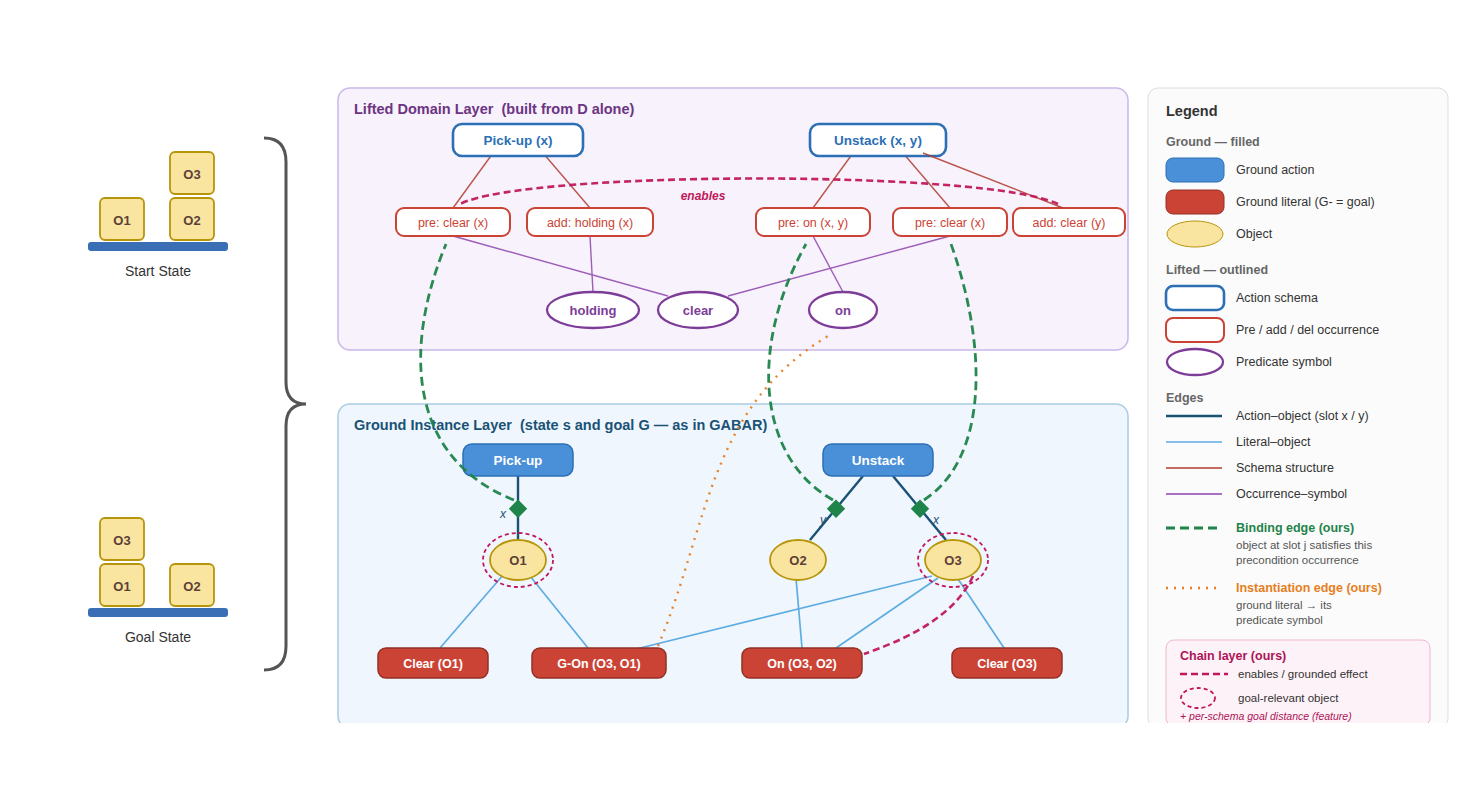
\includegraphics[width=0.98\textwidth]{Figures/gadar_graph_v1.png}
\caption{The \gadar{} representation for a Blocksworld task. The
\emph{ground instance layer} (bottom) is the action-centric graph of the
grounded policy we build on \citep{gabar}: objects, ground literals of the
state and goal (G- prefix), and schema nodes with action--object edges
carrying parameter slots. The \emph{lifted domain layer} (top) is built from
$D$ alone: schemas, their precondition and effect occurrences, and predicate
symbols. \emph{Binding edges} (green, dashed) link an object's slot on an
applicable ground action to the precondition occurrences it satisfies;
\emph{instantiation edges} (orange, dotted) link each ground literal to its
predicate symbol. Filled nodes are ground, outlined nodes lifted. The chain
layer (magenta) is shown by one \emph{enables} edge, one grounded
deletes-true edge, and goal-relevance rings.}
\label{fig:representation}
\end{figure*}

\section{GADAR}

Given a planning instance and its domain description $D$, \gadar{} converts
the pair into a graph, encodes it with a GNN, and constructs a grounded
action with a GRU decoder that first selects an action schema and then each
of its arguments. Encoder and decoder are those of the per-domain policy of
\citet{gabar}; what changes is the graph.

\textbf{Encoder.} Node and edge features are embedded into $d{=}64$
dimensions; $L{=}9$ rounds then update edges, nodes (attention over incoming
edges), and a global node, with skip connections to the input encodings. The
output is one embedding per node, which the decoder ranks.

\subsection{A Domain-Agnostic Graph Representation}

\textbf{Ground instance layer.} The base is GABAR's action-centric graph:
nodes for objects, for ground literals of the current state and the goal
(goal literals flagged), and for action schemas, with a global node; edges
connect literals to their argument objects and schemas to the objects of
their applicable groundings, with parameter positions on the edges
(Figure~\ref{fig:representation}, bottom). The decoder selects among schema
and object nodes present in this input, which is what makes search-free
action construction possible.

\textbf{The graph.} A task $(s, G, D)$ is encoded as $\mathcal{G} = (V, E,
X, R)$ with nodes
\begin{equation*}
V \;=\; O \,\cup\, L \,\cup\, A \,\cup\, \Sigma \,\cup\, Q \,\cup\, \{g\},
\end{equation*}
where $O$ are the objects, $L$ the ground literals of state and goal, $A$
the action schemas, $\Sigma$ the predicate symbols of $D$ (including one
synthetic unary static predicate per declared type, so that typed and
predicate-typed domains present the same structure), $Q$ the
\emph{occurrence nodes} $q_{a,k}$, one per literal occurrence $k$ in the
preconditions and effects of schema $a$, and $g$ a global node. The edges
are typed relations:
\begin{itemize}
\item $E_{\mathrm{lit}} \subseteq L \times O$ and $E_{\mathrm{act}}
  \subseteq A \times O$: literals to their arguments and schemas to the
  objects of their \emph{applicable} groundings, with argument and slot
  positions as edge features;
\item $E_{\mathrm{inst}} \subseteq (L \cup O) \times \Sigma$:
  \emph{instantiation}, each literal to its predicate's symbol and each
  object to its type's symbol;
\item $E_{\mathrm{occ}} \subseteq Q \times (\Sigma \cup A)$: each occurrence
  to its predicate symbol and its schema, carrying its role
  $r(q) \in \{\mathrm{pre}, \mathrm{npre}, \mathrm{add}, \mathrm{del}\}$
  and its argument-to-slot pairs;
\item $E_{\mathrm{bind}} \subseteq O \times Q$, the \emph{binding layer}:
  $(o, q_{a,k})$ whenever some applicable grounding of $a$ places $o$ at a
  slot that occurrence $k$ constrains;
\item $E_{\mathrm{chain}} \subseteq Q \times Q$, the \emph{chain layer}:
  \textit{enables} links an add occurrence to a precondition occurrence of
  the same predicate, \textit{threatens} a delete occurrence to one (with
  the roles exchanged for negative preconditions);
\item $E_{\mathrm{eff}} \subseteq O \times L$, grounded effect edges: for
  each applicable grounding, an add effect equal to an \emph{open} goal atom
  (\textit{achieves-goal}) or a delete effect equal to a \emph{true} atom
  (\textit{deletes-true}) links the grounding's objects to that atom.
\end{itemize}
Node features $X$ concatenate indicator segments: the node's kind, its
arity (clamped at global caps $k_p$, $k_a$) and a static-predicate flag, a
goal flag on literals, on schema nodes a goal-distance one-hot
$\mathrm{gdist}(a) \in \{0, 1, 2, 3{+}\}$ (breadth-first depth over
\textit{enables} from the schemas that add a goal predicate), and on objects
a goal-relevance bit. Edge features $R$ concatenate the relation type with
position, slot, and role indicators. The widths of $X$ and $R$ depend only
on $(k_p, k_a)$; no dimension is the number of schemas, predicates, types,
or objects. One network therefore serves every domain, instances from
different domains batch together, and permuting symbol names leaves
$(X, R)$ unchanged: renaming invariance holds by construction. Every feature
is a flag or a one-hot; the goal distance is bucketed rather than numeric
because no scale is shared across domains, and the same argument makes local
action ranking, rather than value regression, the objective.

\textbf{Why these relations.} $E_{\mathrm{bind}}$ connects what the two
prior lines capture separately: the LLG has lifted preconditions but no
ground actions, and GABAR has ground applicability indexed by per-domain
strings that do not transfer. Binding states why each action is applicable
in $D$'s own vocabulary, and the statement survives renaming of every
symbol. $E_{\mathrm{chain}}$ states directly that schema $A$ produces what
schema $B$ needs; otherwise that relation is a two-hop path through a shared
predicate node whose aggregation loses the producer--consumer pairing.
$E_{\mathrm{eff}}$ places ``this object closes an open goal'' and ``this
object undoes something true'' one hop from the object nodes the decoder
scores. $\Sigma$, $Q$, $E_{\mathrm{occ}}$, and $E_{\mathrm{chain}}$ are
computed once per domain; only $E_{\mathrm{bind}}$, $E_{\mathrm{eff}}$, and
the goal marks are per-state, each linear in the applicable groundings.

\subsection{A Ladder of Domain Conditioning}

We compare five systems, each the previous one plus one group of
components, so that adjacent systems isolate one design decision.
\union{} (the control) keeps GABAR's symbol-identity features, widened to
the union of the training vocabularies: the domain stays in the weights.
\gstruct{} replaces names by structural classes (arity, static or not, goal
or not) but carries no description of $D$. \glift{} adds the lifted domain
layer ($\Sigma$, $E_{\mathrm{inst}}$, and role edges between predicate
symbols and schemas). \gbind{} adds the occurrence nodes and the binding
layer. \gadar{} adds the chain layer, the grounded effect edges, and the
goal features. In addition we remove each of the last four component groups
from \gadar{} alone (``\gadar{} $-$ binding'', and so on). All systems share
one encoder, one decoder, one training procedure, and one executor; only the
graph differs.

\subsection{Action Construction, Training, and Execution}

A GRU selects a schema by scoring schema-node embeddings against its hidden
state, then each argument in turn by scoring object-node embeddings, feeding
every selection back as the next input. The argument loop runs to the
selected schema's arity, read from $D$. No component is sized by the number
of schemas, objects, or predicates: selection is always a dot product
between the decoder state and the embedding of a node in the graph, which is
what lets one network act in a domain whose schemas it has never seen.
Training is supervised cross-entropy against the expert's schema and
argument choices at every state along planner-generated plans; feature
widths are domain-independent, so domains mix freely within a batch.

At test time the decoder keeps the best two schemas and, for each argument,
the best three objects. Each argument's candidates are restricted to
objects that some applicable grounding allows in that slot given the
arguments already chosen, using the applicable groundings the graph is
built from; scores still decide among the legal objects. Without this
restriction, actions with several mutually dependent arguments are
frequently proposed in combinations that do not exist (in Rovers, the
top-ranked proposal was applicable in \todonum{25--44}\% of states), and
execution ends when no proposal is applicable. We apply the same decoding to
every learned system, the per-domain GABAR baseline included.

\section{Experimental Setup}

\textbf{Domains.} We use the eight domains of GABAR: Blocks, Gripper,
Miconic, Visitall, Grid, Logistics, Spanner, and Rovers \citep{gabar,
pddl-generators}. Six declare PDDL types; Grid and Logistics express types
as unary predicates, which the type compilation above makes structurally
equivalent (we verify that typed twins of both domains, with identical
applicable actions, give \todonum{the same} results; supplementary material).

\textbf{Data and splits.} Training sets are 125--312 small instances per
domain (Spanner extended to 8 nuts). Expert plans come from Fast Downward
LAMA-first \citep{fast_downward}. For every domain we build five further
splits of 50 instances each, with sizes in Table~\ref{table:splits}:
\emph{Val-ID} (unseen instances of training size), \emph{Val-OOD}
(moderately larger), and three test bands, \emph{easy}, \emph{medium}, and
\emph{hard}, reaching \todonum{2--3}$\times$ the largest training size or
beyond. Instances are drawn from the existing GABAR test sets, unused
instance pools, and the standard generators \citep{pddl-generators},
de-duplicated against each other and against training, and kept only if
LAMA-first solves them within 600\,s (Spanner's test bands, which are valid
by construction and exceed that limit, excepted). Selection is
deterministic: round-robin over sizes within a band, existing test
instances first.

\begin{table}[t]
\centering
\small
\caption{Instance sizes per split (50 instances each).}
\label{table:splits}
\setlength{\tabcolsep}{3pt}
\begin{tabular}{@{}lcccccc@{}}
\toprule
Domain (size) & Train & Val-OOD & Easy & Medium & Hard \\
\midrule
Blocks (blocks) & 6--9 & 10 & 11--20 & 21--30 & 31--40 \\
Gripper (balls) & 5--25 & 26--30 & 31--50 & 51--75 & 76--100 \\
Miconic (pass.) & 1--12 & 13--19 & 20--40 & 41--60 & 61--100 \\
Visitall (cells) & 9--49 & 50--64 & 65--144 & 145--225 & 226--400 \\
Grid (cells) & 9--63 & 64--80 & 81--100 & 101--125 & 126--154 \\
Logistics (cities) & 5--13 & 14--15 & 16--20 & 21--25 & 26--30 \\
Spanner (nuts) & 3--8 & 9--10 & 11--12 & 13--14 & 15--16 \\
Rovers (waypoints) & 3--12 & 13--15 & 16--30 & 31--50 & 51--70 \\
\bottomrule
\end{tabular}
\end{table}

\textbf{Experiments.} (i)~\emph{Zero-shot}: leave-one-domain-out, a policy
trained on seven domains is tested on the eighth, whose predicates,
schemas, and objects it has never seen. (ii)~\emph{In-domain}: \gadar{} and
GABAR each trained on one domain, and one \gadar{} policy trained on all
eight, tested on the test bands of their training domains. (iii)~The
ladder, on three folds (Blocks, Logistics, and Visitall held out).

\textbf{Checkpoint selection.} Every model is trained for 500 epochs with a
snapshot every 50. We report the snapshot with the lowest teacher-forced
cross-entropy on the Val-OOD instances of its \emph{training} domains; for
several training domains, the mean over domains of each domain's loss
relative to its own best snapshot, so that domains with larger losses do not
dominate. The held-out domain contributes nothing to selection. We select on
loss rather than coverage because Val-OOD coverage saturates: most
snapshots solve every Val-OOD instance.

\textbf{Baselines.} \union{} is the primary control: identical data,
architecture, training, decoding, and execution, with only the
representation different. GABAR \citep{gabar} is re-trained under the same
protocol (data, selection, decoding) as the per-domain reference. Two
non-learned baselines use the same executor: \emph{random} choice among
applicable actions, and a \emph{goal-feature rule} that ranks applicable
actions by the information \gadar{}'s chain layer encodes (achieves an open
goal, then does not delete a goal atom, then schema goal distance, then
goal-relevant arguments); it measures what the network adds to the
features it is given.

\textbf{Metrics and implementation.} Coverage is the percentage of
instances solved within 500 steps. All learned systems use batch size 64,
learning rate $5\cdot10^{-4}$, and the encoder and decoder settings of
GABAR. Results are for \todonum{one seed; three seeds with standard
deviation in the final version}. Training ran on single NVIDIA V100 (32\,GB),
RTX~8000, A40, and H100 GPUs with \todonum{4--8} CPU cores and 32--64\,GB of
memory; no per-instance time limit is imposed on the policy beyond the step
bound. Software: Fast Downward commit 83dfcd7, PyTorch 2.6.0, PyTorch
Geometric 2.6.1, and a modified pddlgym; code and splits are in the
supplementary material.

\section{Results}

\begin{table}[t]
\centering
\small
\caption{Zero-shot coverage (\%) on the hard test band of each held-out
domain, never seen in training. Random and Rule: non-learned baselines under
the same executor. Easy and medium bands: supplementary material.}
\label{table:zeroshot}
\begin{tabular}{@{}lcccc@{}}
\toprule
Held out & Random & Rule & \union{} & \gadar{} \\
\midrule
Blocks    & \todonum{} & \todonum{} & \todonum{} & \todonum{} \\
Gripper   & \todonum{} & \todonum{} & \todonum{} & \todonum{} \\
Miconic   & \todonum{} & \todonum{} & \todonum{} & \todonum{} \\
Visitall  & \todonum{} & \todonum{} & \todonum{} & \todonum{} \\
Grid      & \todonum{} & \todonum{} & \todonum{} & \todonum{} \\
Logistics & \todonum{} & \todonum{} & \todonum{} & \todonum{} \\
Spanner   & \todonum{} & \todonum{} & \todonum{} & \todonum{} \\
Rovers    & \todonum{} & \todonum{} & \todonum{} & \todonum{} \\
\midrule
Mean      & \todonum{} & \todonum{} & \todonum{} & \todonum{} \\
\bottomrule
\end{tabular}
\end{table}

\begin{table}[t]
\centering
\small
\caption{In-domain coverage (\%) on the hard test band. GABAR and
\gadar{}$_1$: one model per domain; \gadar{}$_8$: one model for all eight
domains. Same splits, selection rule, and decoding for all three.}
\label{table:indomain}
\begin{tabular}{@{}lccc@{}}
\toprule
Domain & GABAR & \gadar{}$_1$ & \gadar{}$_8$ \\
\midrule
Blocks    & \todonum{} & \todonum{} & \todonum{} \\
Gripper   & \todonum{} & \todonum{} & \todonum{} \\
Miconic   & \todonum{} & \todonum{} & \todonum{} \\
Visitall  & \todonum{} & \todonum{} & \todonum{} \\
Grid      & \todonum{} & \todonum{} & \todonum{} \\
Logistics & \todonum{} & \todonum{} & \todonum{} \\
Spanner   & \todonum{} & \todonum{} & \todonum{} \\
Rovers    & \todonum{} & \todonum{} & \todonum{} \\
\midrule
Mean      & \todonum{} & \todonum{} & \todonum{} \\
\bottomrule
\end{tabular}
\end{table}

\begin{table}[t]
\centering
\small
\caption{The ladder on three folds: zero-shot coverage (\%) on the held-out
domain's hard band, and in-domain coverage averaged over the seven training
domains' hard bands (ID).}
\label{table:ladder}
\setlength{\tabcolsep}{3.5pt}
\begin{tabular}{@{}lcccc@{}}
\toprule
& Blocks & Logistics & Visitall & ID \\
\midrule
\union{}                  & \todonum{} & \todonum{} & \todonum{} & \todonum{} \\
\gstruct{}                & \todonum{} & \todonum{} & \todonum{} & \todonum{} \\
\glift{}                  & \todonum{} & \todonum{} & \todonum{} & \todonum{} \\
\gbind{}                  & \todonum{} & \todonum{} & \todonum{} & \todonum{} \\
\textbf{\gadar{}}         & \todonum{} & \todonum{} & \todonum{} & \todonum{} \\
\midrule
\gadar{} $-$ binding      & \todonum{} & \todonum{} & \todonum{} & \todonum{} \\
\gadar{} $-$ chain        & \todonum{} & \todonum{} & \todonum{} & \todonum{} \\
\gadar{} $-$ effect edges & \todonum{} & \todonum{} & \todonum{} & \todonum{} \\
\gadar{} $-$ goal features& \todonum{} & \todonum{} & \todonum{} & \todonum{} \\
\bottomrule
\end{tabular}
\end{table}

% Each paragraph answers one question with one comparison. Text is written
% once the numbers exist; do not state a direction before it is measured.

\textbf{Does the domain need to be in the input? (\union{} vs.\ \gadar{},
Table~\ref{table:zeroshot}.)} \todonum{Fill from Table 1.}

\textbf{Does the network add to its features? (Rule vs.\ \gadar{}.)}
\todonum{Fill from Table 1.}

\textbf{What makes zero-shot transfer work? (The ladder,
Table~\ref{table:ladder}.)} Each step answers one question: whether names
transfer (\union{} to \gstruct{}), whether the description of $D$ helps
(\gstruct{} to \glift{}), and whether binding makes it actionable (\glift{}
to \gbind{}, and \gadar{} $-$ binding). \todonum{Fill from Table 3.}

\textbf{Does describing symbols by their roles cost in-domain coverage?
(GABAR vs.\ \gadar{}$_1$, Table~\ref{table:indomain}.)} \todonum{Fill from
Table 2.}

\textbf{Does one policy serve all domains? (\gadar{}$_1$ vs.\ \gadar{}$_8$.)}
\todonum{Fill from Table 2.}

\textbf{Where does zero-shot transfer fail?} \todonum{Per-domain analysis;
structurally alike schemas with different roles (Logistics' truck and
airplane actions) are one expected cause.}

\textbf{Limitations.} The representation covers STRIPS with types and
negative preconditions. Conditional effects (e.g., Caldera), quantified
conditions, and equality constraints are outside it; so are action schemas
beyond the decoder's argument cap \todonum{(Organic Synthesis has schemas
with up to 31 parameters)}. Grounding is per visited state, not per task,
but its cost grows with the number of applicable actions.

\section{Conclusion}

\todonum{Write once the results are in.} \gadar{} is a policy for classical
planning that takes the domain description as input and constructs grounded
actions in domains never seen in training, without search. Few-shot
adaptation, lifted successor generation, richer PDDL fragments, and
probabilistic settings remain future work.

\bibliography{references}

\end{document}
